%% LyX 1.3 created this file.  For more info, see http://www.lyx.org/.
%% Do not edit unless you really know what you are doing.
\documentclass[english]{article}
\usepackage{pslatex}
\usepackage[T1]{fontenc}
\usepackage[latin1]{inputenc}
\usepackage{graphicx}
\IfFileExists{url.sty}{\usepackage{url}}
                      {\newcommand{\url}{\texttt}}

\makeatletter
\usepackage{babel}
\makeatother
\begin{document}

\title{Documentation on smoothing\\
Draft}


\author{Tchize}


\date{Seven of July 2003}

\maketitle

\section{Introduction}

The crossfire graphical interface and internal map handling relies
on a map made of square. No object can lies between squares. A typical
square has the size of a standing player or other humano�d sized creature
(Goblins, Orcs, Gnolls, Dwarvens, Elves, ...). This lead to an awfull
interface concerning terrains transitions (Sea shores, road borders,
mountains, a.s.o)

There are 2 ways to get rid of this problem:

\begin{itemize}
\item Suppress the square by square behaviour of map handling. This means
rework half of crossfire code and redraw all maps
\item Use some magic illusion.
\end{itemize}

\section{What is smoothing}

Large discussions in the cf-devel mailing list was around a document
on terrain transitions available on \url{http://www.gamedev.net/reference/articles/article934.asp}.
It explains a way of handling terrain transition in cases like the
one of crossfire. 

Consider the smoothing in crossfire as the ability for an object to
draw itself partially above the surrounding squares. For example,
grass could overlap just a bit the road next to it, a moutain would'nt
end abruptly but instead would have some hills above the neighbor
sand.


\section{How to smooth?}

Next of this document is divided in 2 parts. Drawers should be interrested
only in first part while developpers may be interested in both parts.


\subsection{Basic smoothing}

Basically, there need to be some order for smoothing. If everything
draws itself above every surrounding square, we would end up with
some awful bunch of crapy disgusting mixture of color (a Picasso or
alike).

So, we comme to the

\begin{flushright}\textbf{First Rule}\end{flushright}

An object O may draw itself above a neighbor object V if, and only
if, 0 as a <<smoothlevel>> higher than V. See the things like that:

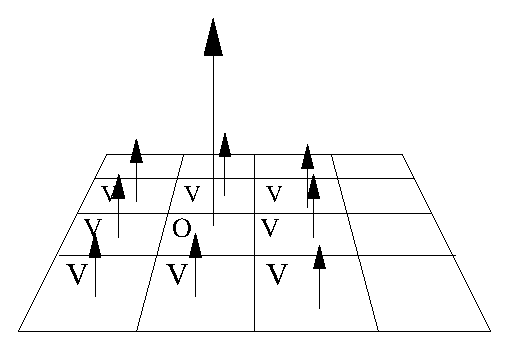
\includegraphics{img/smoothlevel.eps}

O in the exampel picture has a higher priority than V so O will overlap
V a bit but V will not overlap O.

The smoothlevel is an integer value ranging from 0 (overlap nothing)
to 255 (overlap above everything except other objects having also
smoothlevel of 255). This is important to consider when you are going
to give the smoothing ability to new objects. Let's say, for example,
you want to add this ability to mountains. Let's imagine has a smoothlevel
of 10 and trees have a smoothlevel 100 (just imagine, at time writing
this doc, nothing fixed yet). Now let's say you want the moutains
above the grass but, for graphical reasons, you want the trees above
the mountains. You Choose a value between 10 and 100, not included.
But mountains is a thing that goes above a lot of thing (grass, hills,
swamps, brush, rocks, desert,...). So to keep the place for adding
new elements in the future, you rather choose a high value for mountains
(90 seems a good value according to these conditions).

So now you have chosen the smoothlevel for the mountain. What on hell
are you supposed to draw? You know what overlap what is decided by
smoothlevel. But the graphics used during the smoothing is the 

\begin{flushright}\textbf{Second Rule}\end{flushright}

The picture used to draw a given object depend on the face of the
object. All objects using the grass face, for example, if they have
a smoothlevel higher than 0, will be smooth using the same pictures.
So you will bind with the picture grass.111 a set of pictures telling
the client what to draw when smoothing an object having the face grass.111.
Take a look at the canvas below:

\noindent 
\includegraphics[%
  width=1.0\columnwidth]{img/canvas_smooth.eps}

Each square have a size of 32x32, which is the size used by the current
image sets. This canvas handles all cases of corner, borders, L shaped,
U shaped and O shaped transitions. The picture is made of 16 elements
by 2. The first line is all broder related transition. The second
line is corner related transitions. Here is an example picture for
grass (yeah really need someone to rework it):

\begin{flushleft}
\includegraphics[%
  width=1.0\columnwidth]{img/sgrass.base.111.eps}\end{flushleft}

The picture is named sgrass.base.111.png and located in the ground/smooth/grasslike
directory of archetype. Ok, now you have a picture for smoothing grass,
you have a smoothlevel for grass. There is only one last thing to
do:

\begin{flushright}\textbf{Final Rule}\end{flushright}

Tell the server which picture to send the client. There is, in the
server CVS directory a file named lib/smooth. This file is where you
set this information. Each line in the file beginning with \emph{\#}
is a comment. Other line should be made of 2 elements:

The first is the picture you want to smooth (here it is grass.111%
\footnote{Please note we suppressed the .png and the .base. elements of grass.base.111.png
filename. Since what the server needs is the internal names. Take
care of this. If the new picture you drawn didn't appear on the GUI,
this is perhaps due to error in this file. And don't forget to copy
this file, afterwards, to the install directory of server, using a
make~install.%
}) the second is the 512x64 picture drawn at rule 2 and used when smoothing.
And example line might be as follow:

\texttt{grass.111 sgrass.111}

The entry default\_smoothed.111 is used when the server can not find
an appropriate entry for an object. This correspond to the black canvas
above so mapmakers or drawers can see immediatly there is a problem.

Now, drawers know everything. Coders might want to read following
part.


\subsection{Smoothing in the code}

Guess what...

TODO
\end{document}
